%!TEX root = ../zeeman.tex
\begin{figure}[H]{}
\centering
\vspace{-10pt}
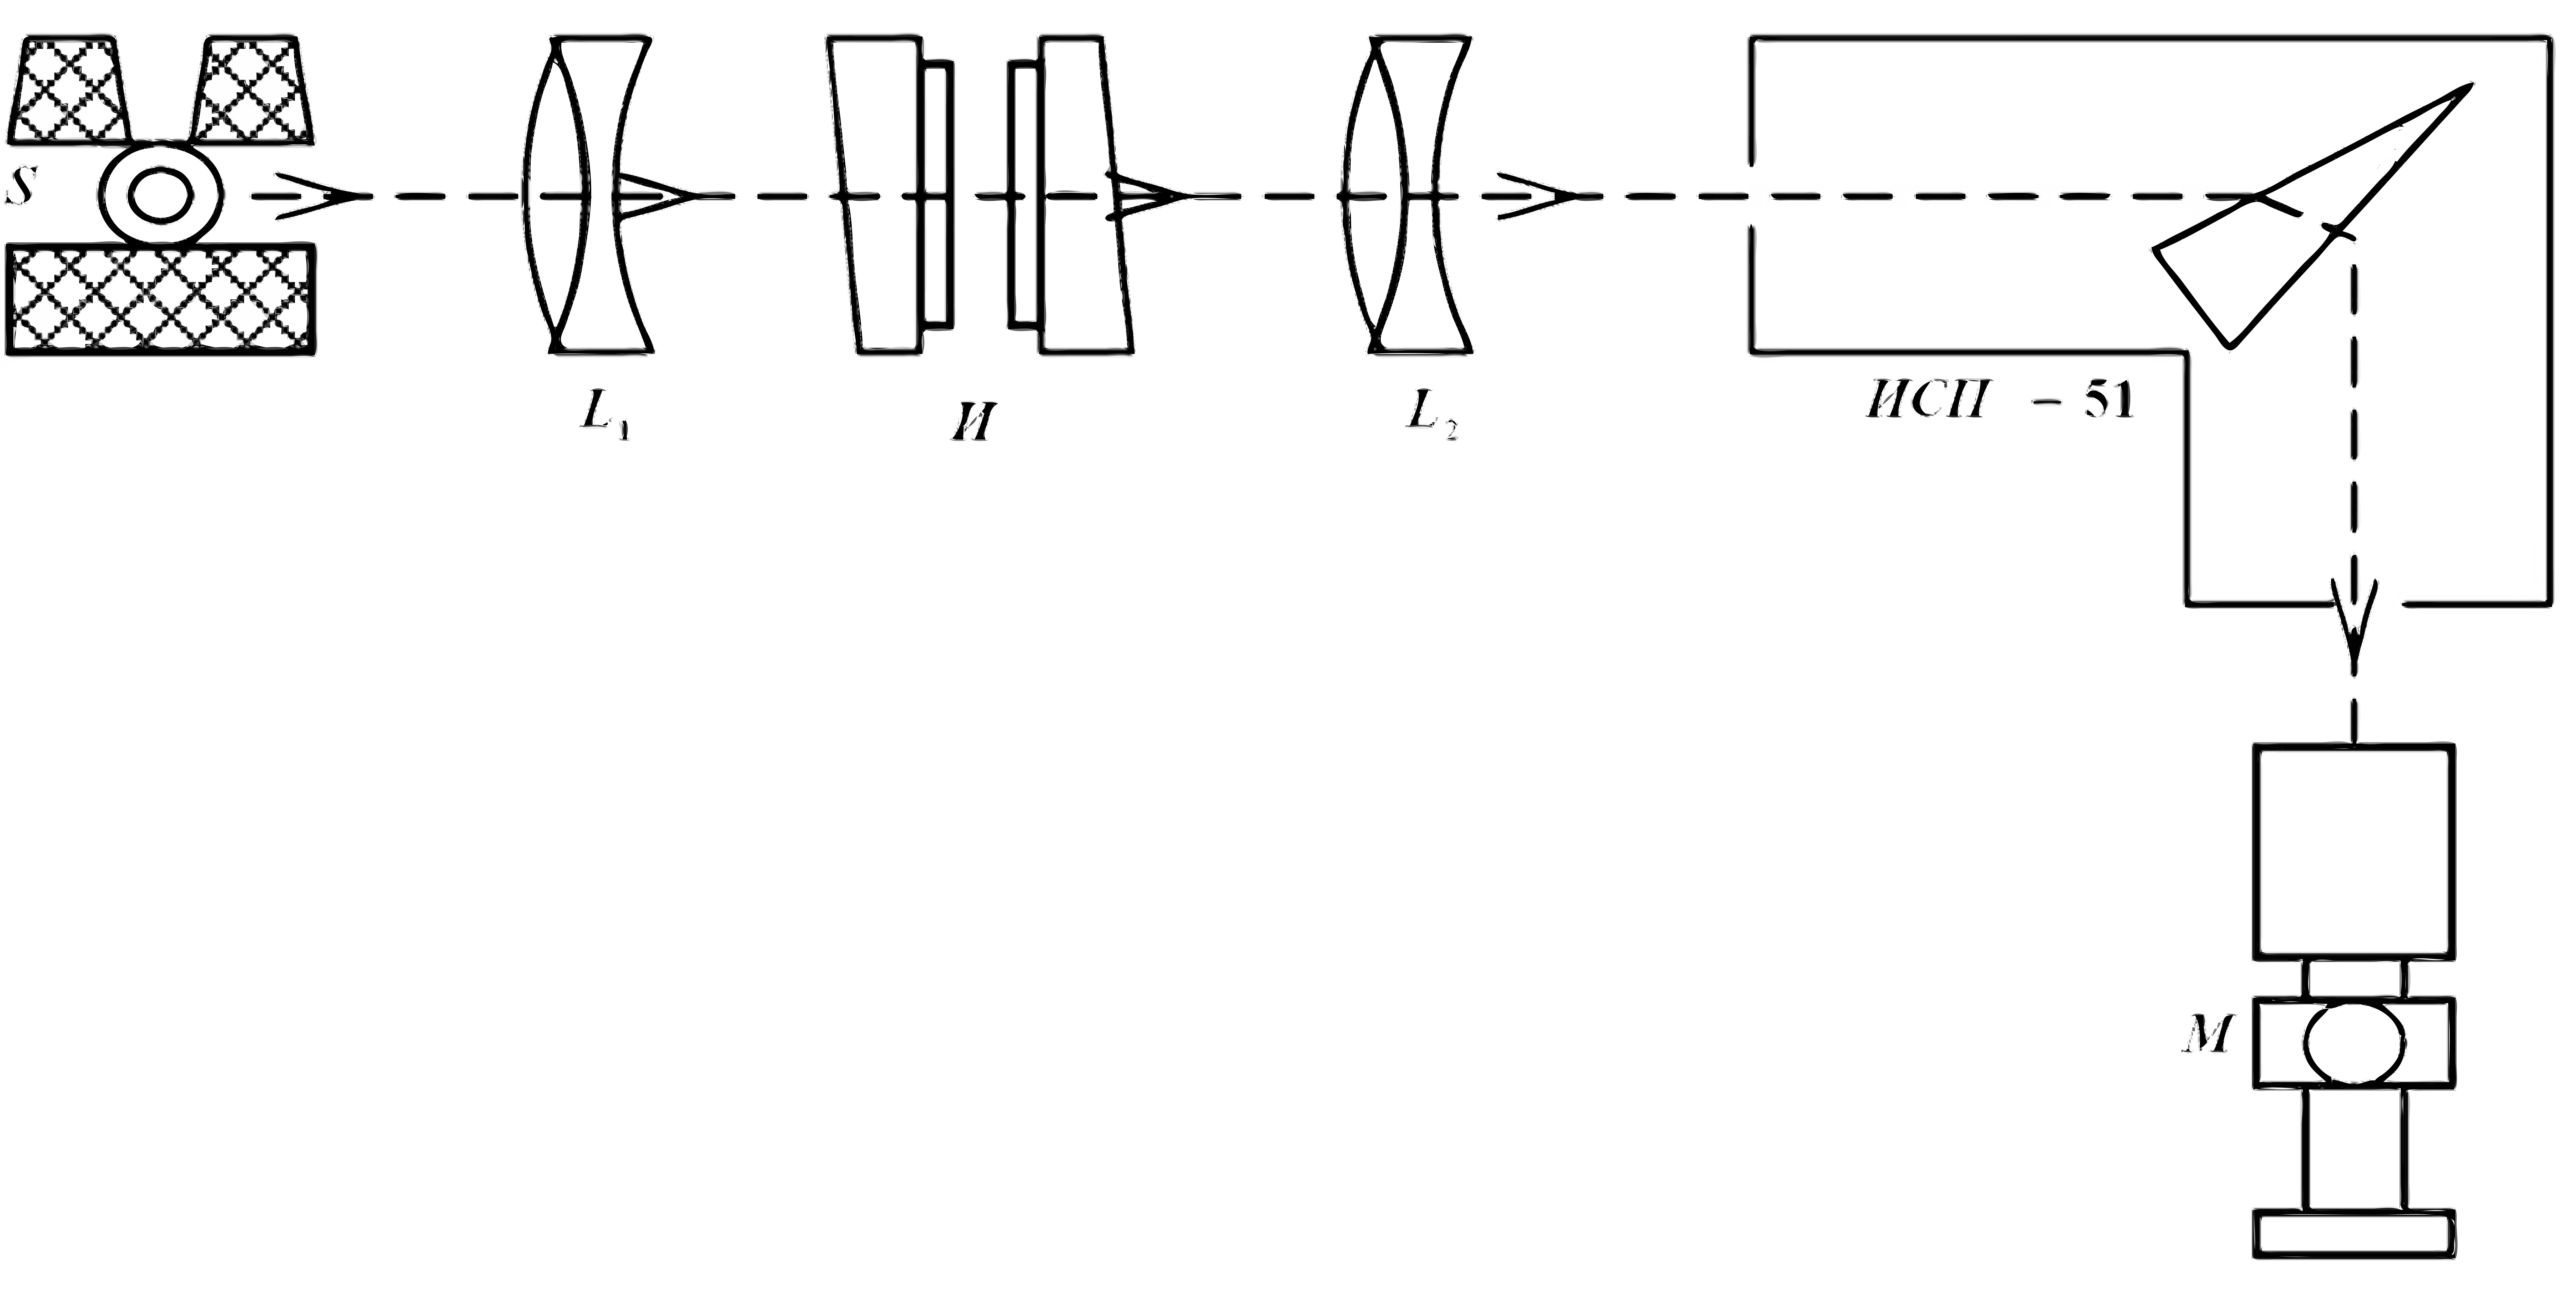
\includegraphics[width=0.9\textwidth]{fig/fig6.jpg}
\vspace{-40pt}

\caption{Cхема экспериментальной установки} \label{fig:6}
\end{figure}

Целью данной работы является изучение эффекта Зеемана на примере спектра излучения $Ne$ с помощью \textbf{интерферометра Фабри-Перо (ИФП)}.

Схема экспериментальной установки приведена на \ref{fig:6}. Здесь $S$ - газосветная трубка, помещенная между полюсами поворачивающегося электромагнита, \textbf{И-ИФП}, $L_1$ и $L_2$ - ахроматические линзы, \textbf{ИСП-51} - призменный спектрограф, \textbf{T} - короткофокусная зрительная трубка, \textbf{M} - окулярный микрометр. 

\textbf{ИФП} является многолучевым интерферометром высокой разрешающей способности. Он состоит из двух прозрачных клиновидных пластин (см. рис. \ref{fig:7}), внутренние поверхности которых ограничивают плоскопараллельный слой воздуха. На эти поверхности нанесено диэлектрическое покрытие, обеспечивающие энергетический коэффициент отражения $\rho$, близкий к единице. 

\begin{wrapfigure}{h}{0.4\textwidth}

\begin{center}
\vspace{-25pt}
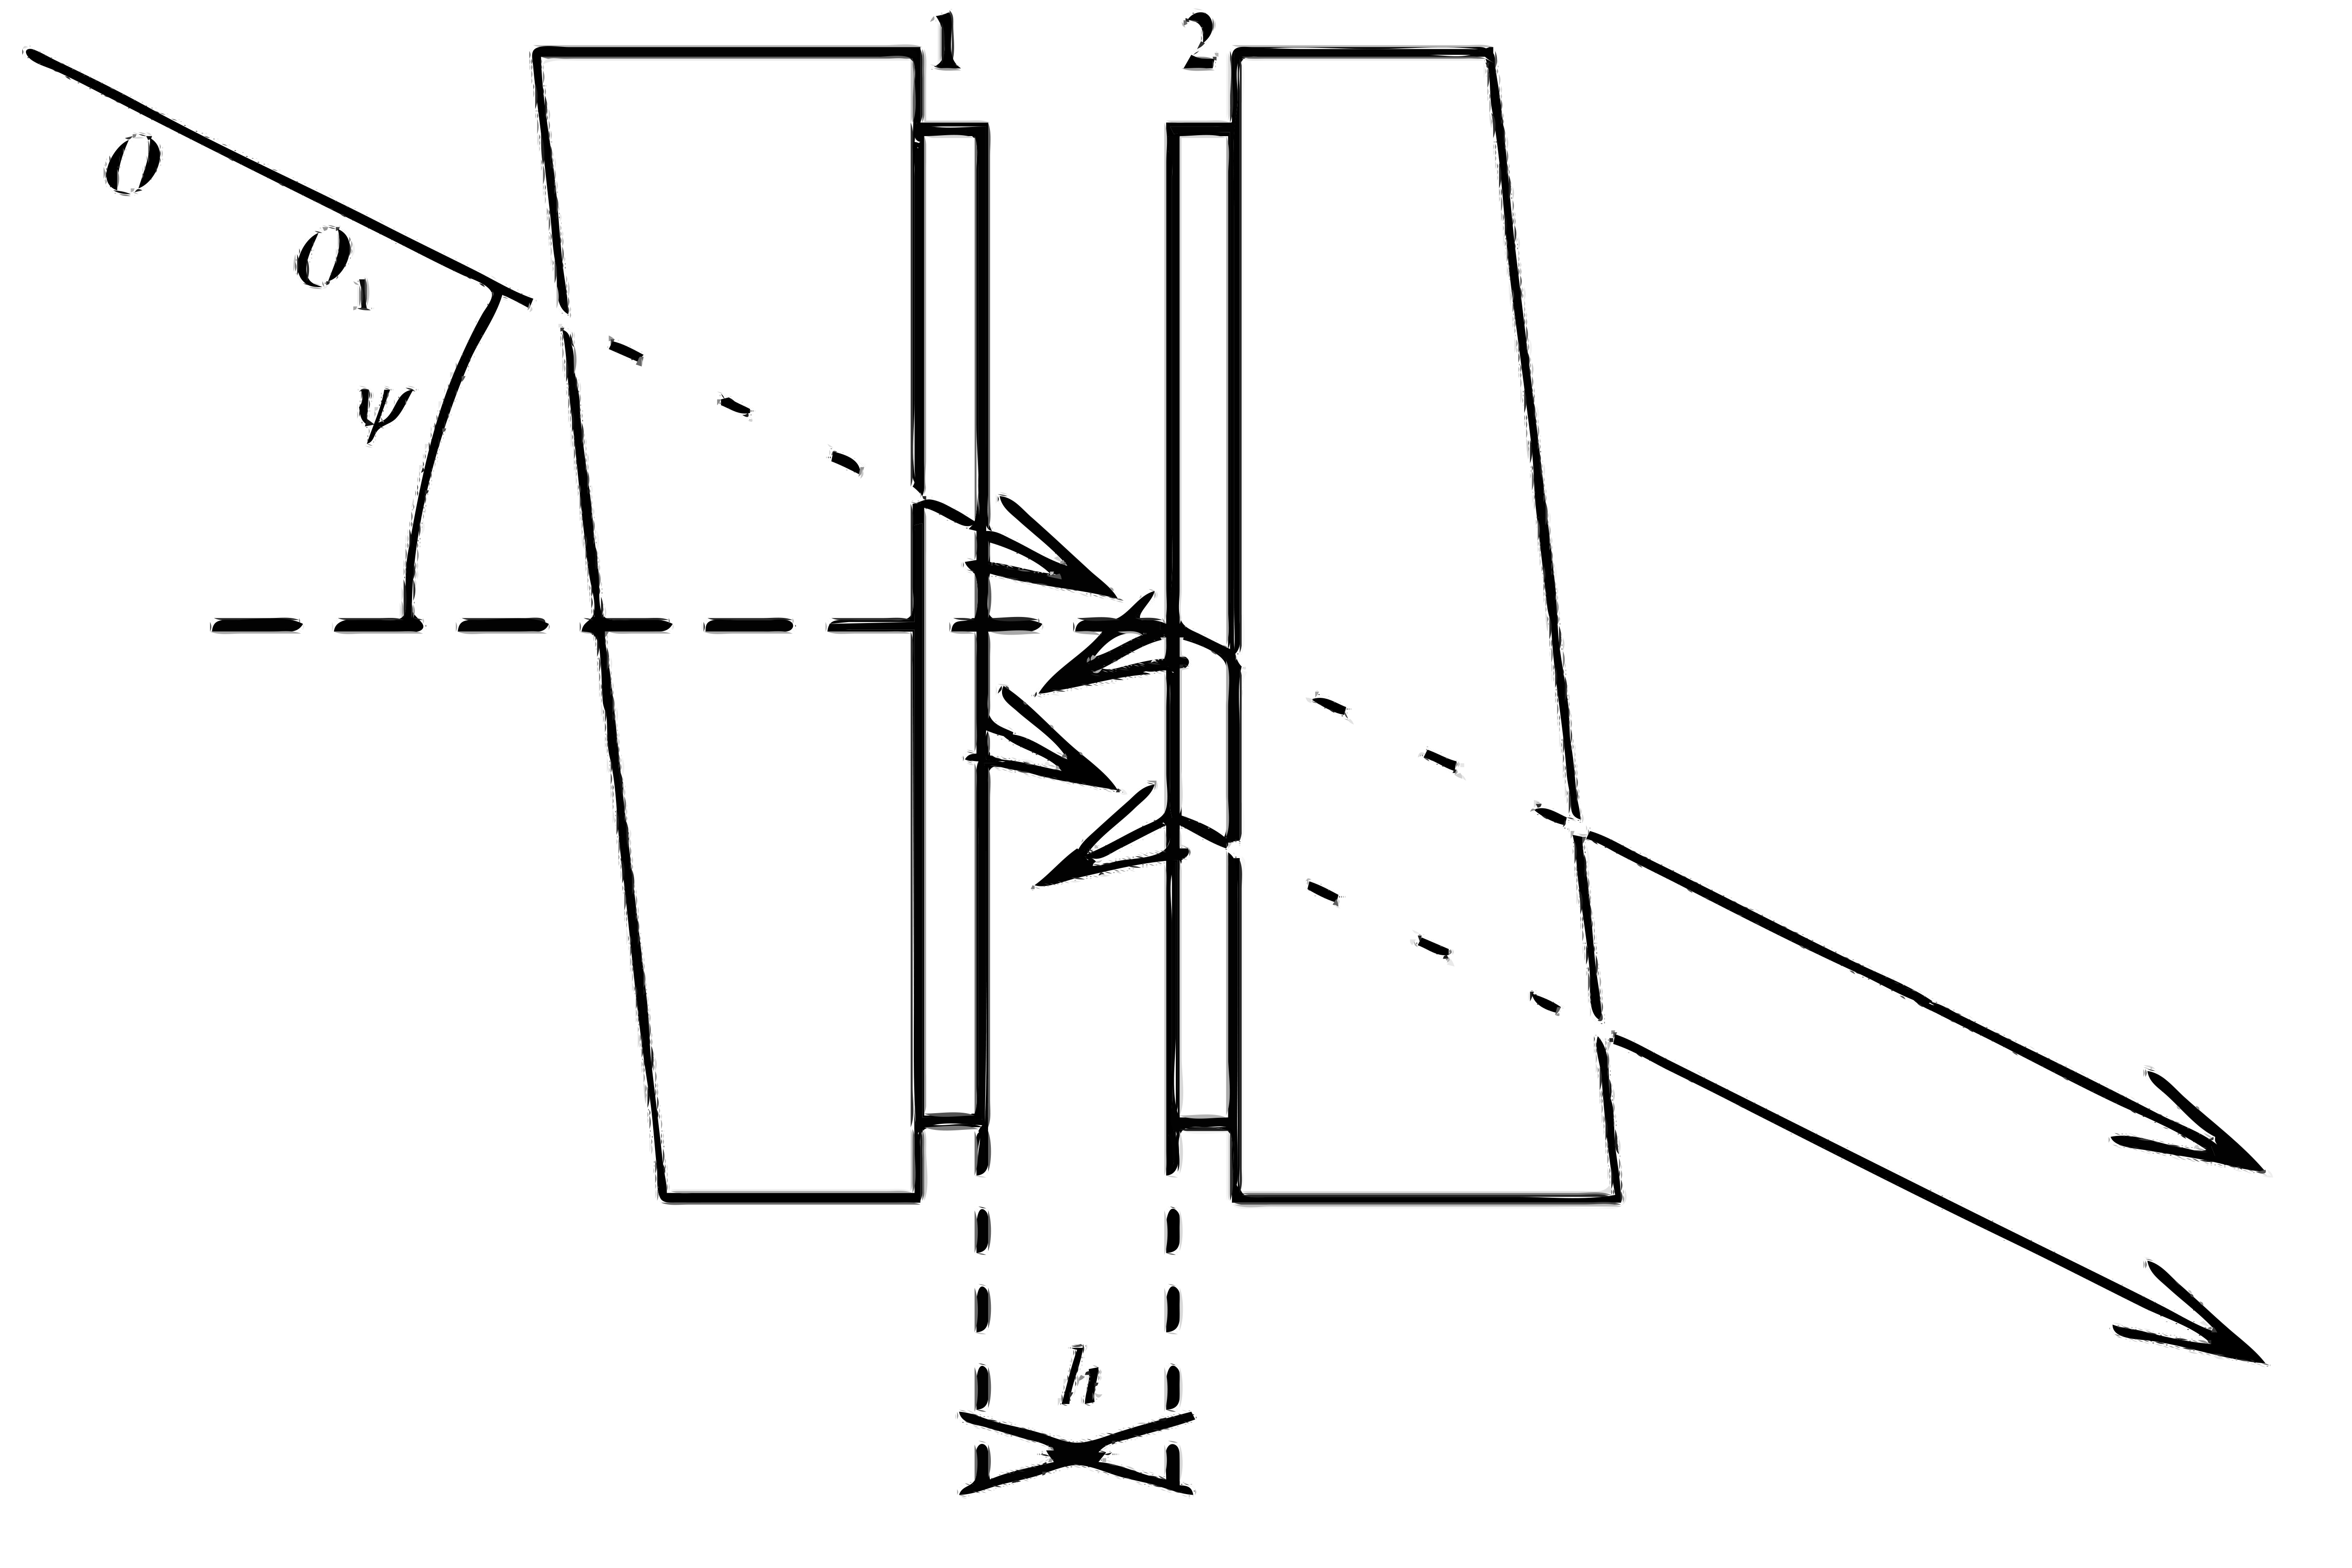
\includegraphics[width=0.4\textwidth]{fig/fig7.jpg}
\caption{Интерферометр Фабри-Перо} \label{fig:7}
% \vspace{-40pt}

\end{center}

\end{wrapfigure}

Луч $OO_1$, вошедший в интерферометр и многократно отразившийся от зеркальных поверхностей 1 и 2, образует ряд проходящих параллельно лучей с постоянной разностью хода 
\begin{equation}
	\Delta=2h \cos \Psi,
\end{equation} где $h$ толщина воздушного слоя, $\Psi\ll 1$-- угол падения света в зазоре. 

Объектив, установленный за \textbf{ИФП}, формирует \textbf{линии равного наклона}, представляющие собой систему концентрических колец. Угловые радиусы $\Psi_1$ колец Фабри-Перо для длины волны $\lambda$ удовлетворяют условию интерференционных максимумов 
\begin{equation}
\label{eq:24}
	2h \cos \Psi_i = m_i \lambda=m_0 \lambda \cos \Psi_i,
\end{equation}

где $m_i$ - порядок интерференции (большое целое число, так как $h \gg \lambda$); $m_0=2h/\lambda$ - максимальный порядок интерференции, получающийся при $\Psi=0$, то есть в центре картины; $i=1, 2, 3,\dots$ - номер кольца по порядку от центра картины. 



Легко показать, что диаметры колец Фабри-Перо описываются формулой: 
\begin{equation}
	\label{eqL25}
	d_i^2=\frac{4 f^2 \lambda (i-1+\varepsilon_{\lambda})}{h}
\end{equation}
где $f$ - фокусное расстояние объектива $\varepsilon_{\lambda} \in [0;1]$ - так называемая дробная доля порядка интерференции в центре колец, определяемая равенством 
\begin{equation}
	\label{eq:26}
	m_0 - m_i=i-1+\varepsilon_{\lambda}.
\end{equation}

 Характерными особенностями \textbf{ИФП} как спектрального прибора являются высокая \textbf{разрешающая способность}
 \begin{equation}
 	\label{eq:27}
 	R=\frac{m_i \pi \sqrt{\rho}}{1-\rho}
 \end{equation}
 
и малая \textbf{дисперсионная область}
\begin{equation}
	\label{eq:28}
 	\Delta \lambda_{\text{своб}}=\frac{\lambda^2}{2h \cos \Psi}.
 \end{equation} 

Как правило, это делает необходимым использование дополнительного \textbf{монохроматора}. В нашем случае им служит \textbf{призменный спектрограф ИСП-51}.
\begin{figure}[H]
	\begin{center}
	% \vspace{}
	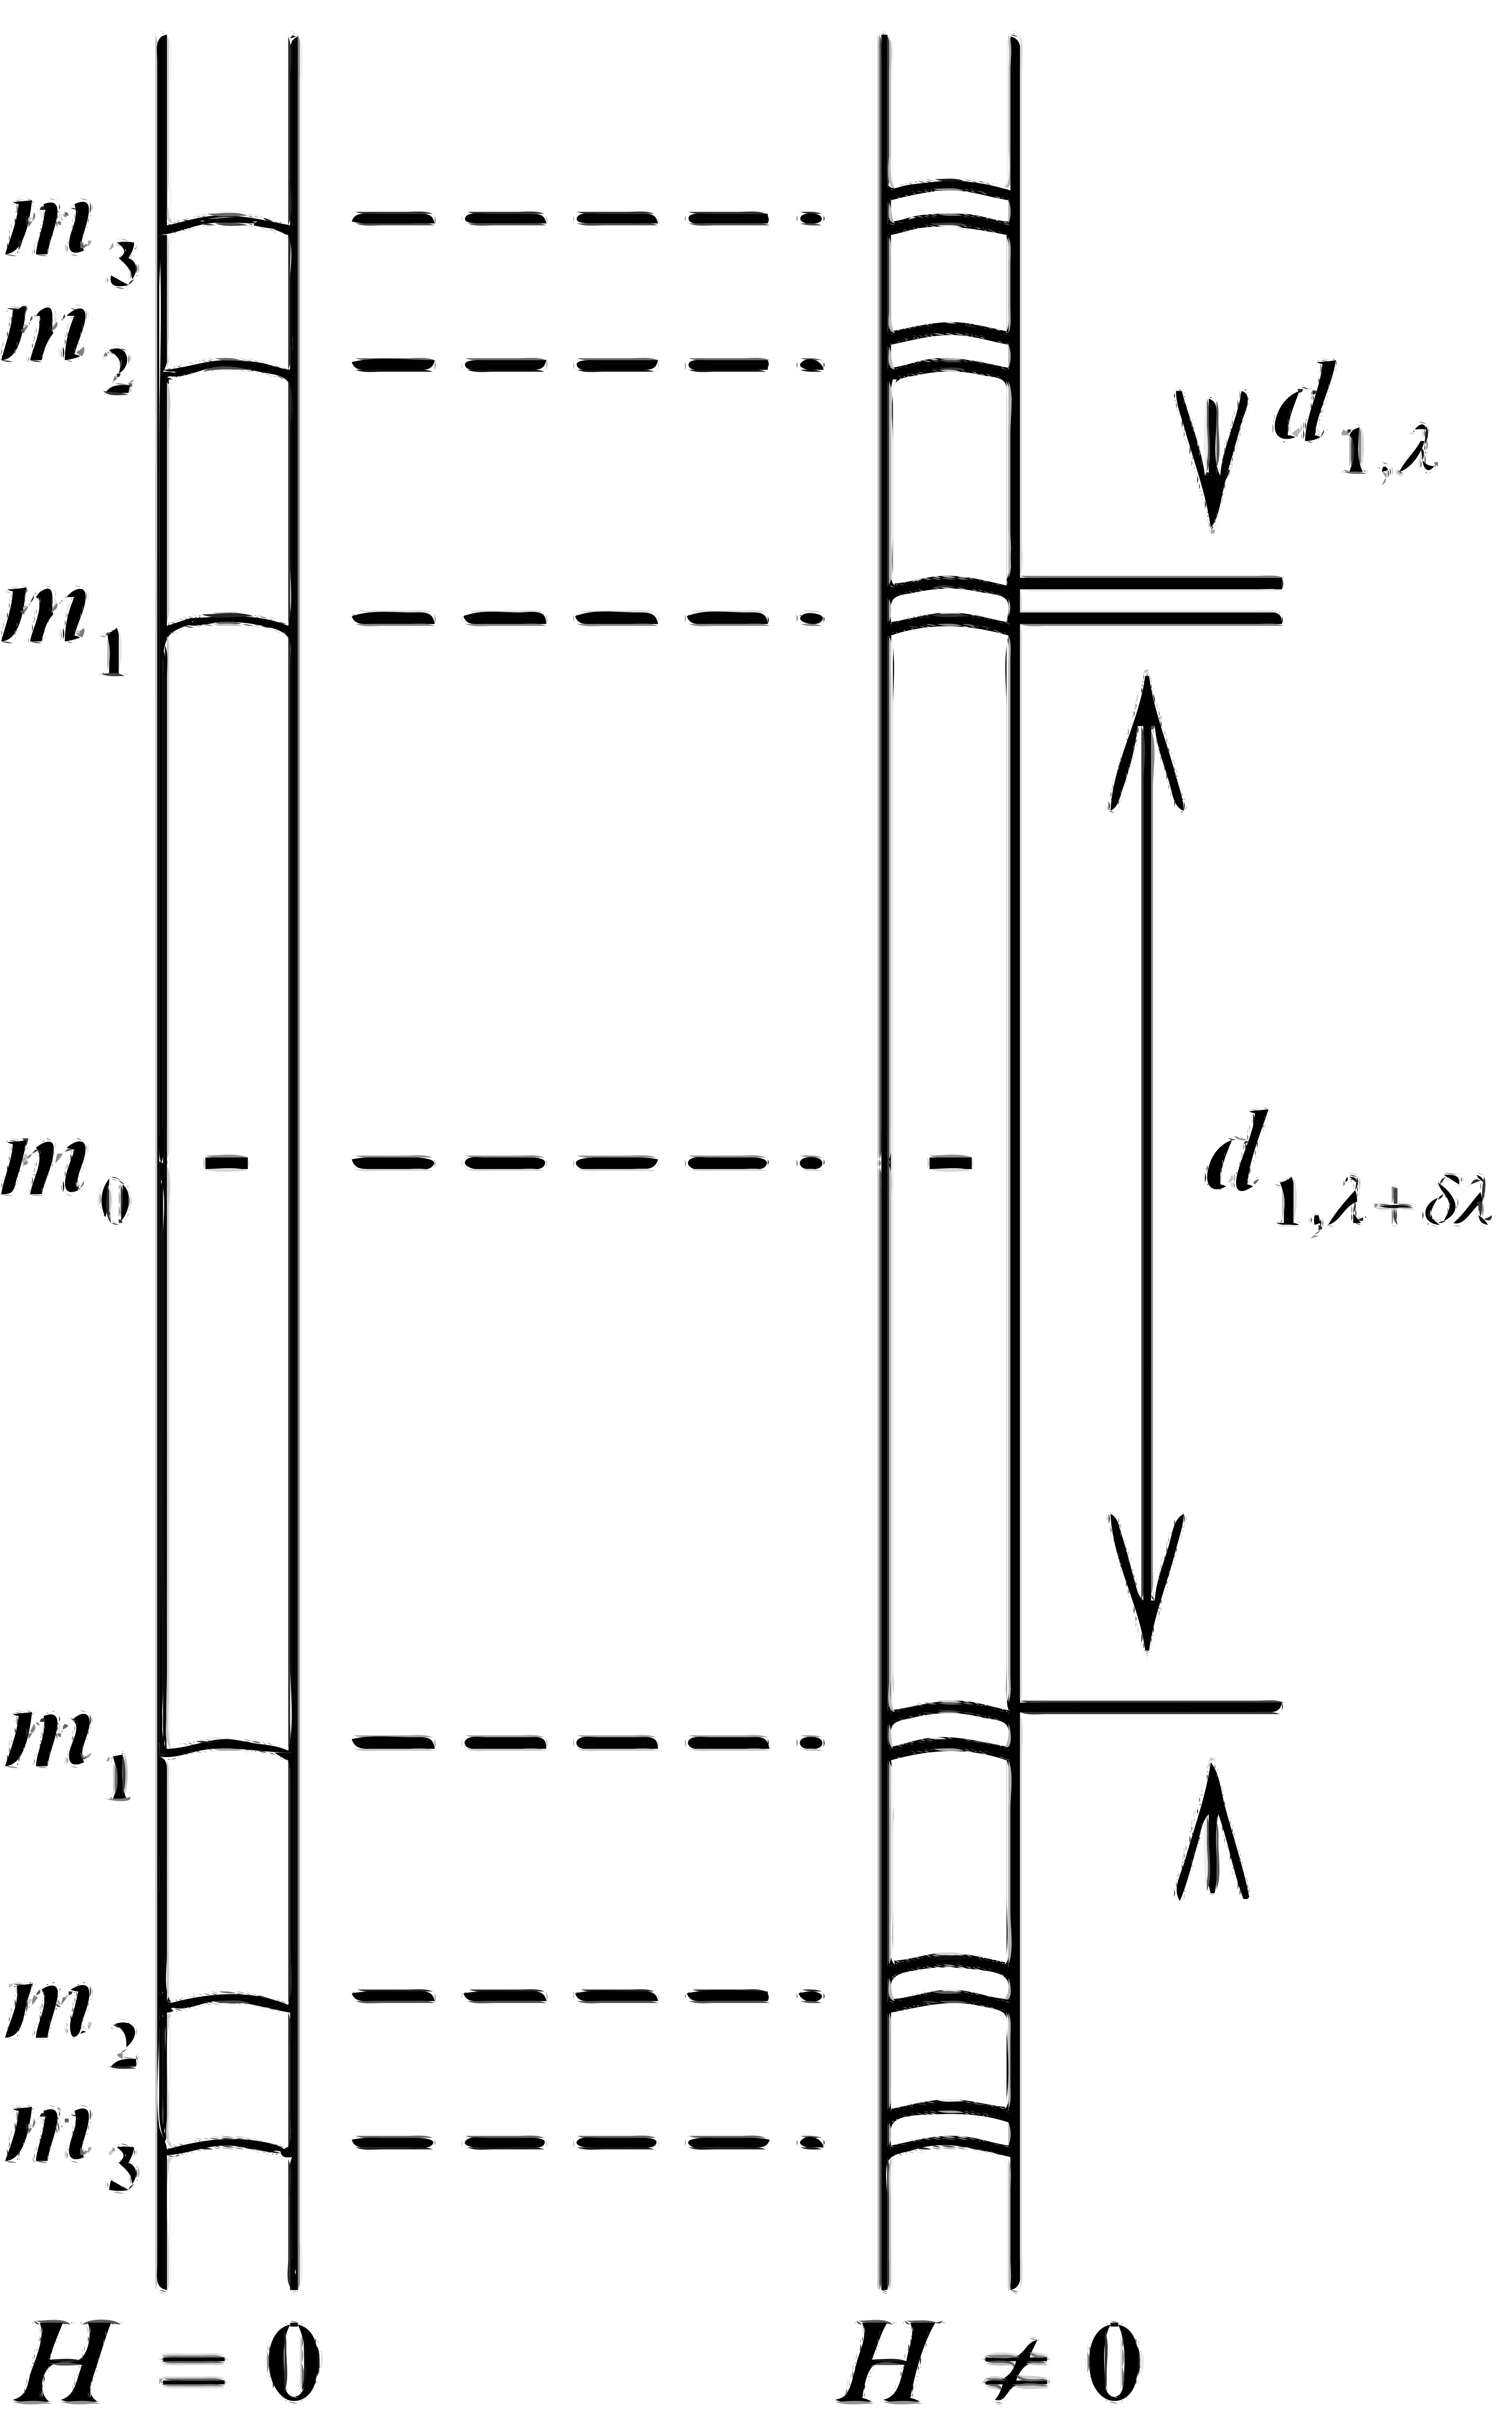
\includegraphics[width=0.4\textwidth]{fig/fig8.jpg}
	% \vspace{-10pt}
	\caption{Вид спектральных линий в выходной плоскости спектрографа}\label{fig:8}
\end{center}

\end{figure}
ИФП устанавливается таким образом, чтобы плоскость локализации колец Фабри-Перо совместилась с плоскостью входной щели спектрографа. Щель вырезает из колец узкую вертикальную полоску. Таким образом, спектрограф разлагает свет в горизонтальной плоскости, а ИПФ - вдоль вертикальной входной щели спектрографа. В результате наблюдения картина, состоящая из ряда светлых вертикальных полосок, прорезанных яркими дугами колец Фабри-Перо. Положение колец определяет тонкую структуру соответствующей спектральной линии. 

Параллельные пучки лучей, вышедших из интерферометра Фабри-Перо (\ref{fig:7}) в фокальной плоскости объектива образуют систему концентрических колец -- линии равного наклона. Однако в окуляр зрительной трубы видны лишь небольшие участки дуг этих колец, соответствующие различным спектральным линиям неона. Для определения величины расщепления $\delta\lambda$ проводят измерения либо диаметров колец, либо лишь разностей их радиусов. В последнем случае установку надо настроить так, чтобы наблюдались лишь верхние (либо нижние) части колец. При этом можно сделать увеличение трубы больше, что облегчает измерение дуг $x_{\lambda-\Delta \lambda},x_{\lambda},x_{\lambda+\Delta \lambda}$ (см. рис. \ref{fig:9}) и уменьшает ошибки измерений.

Получим формулу для расчёта величины $\delta \lambda$. Условие наблюдения интерференционных колец выражается формулой (\ref{eq:24}). Из рис. \ref{fig:10}  с учётом малости угла $\Psi$ для радиуса кольца $R$ найдем
\begin{equation}
	\label{eq:29}
	R\approx f\Psi,
\end{equation}
где $f$-- фокусное расстояние объектива.


Для разностей радиусов \ref{fig:9} из соотношения \ref{eq:29} получим 
\begin{gather}
	\label{eq:30}
	\Delta R_m \approx f \delta \Psi_m \text{ и } \Delta R_{\lambda} \approx f \delta \Psi_{\lambda} 
\end{gather}
%рис 9
\begin{figure}[H]
	\centering
	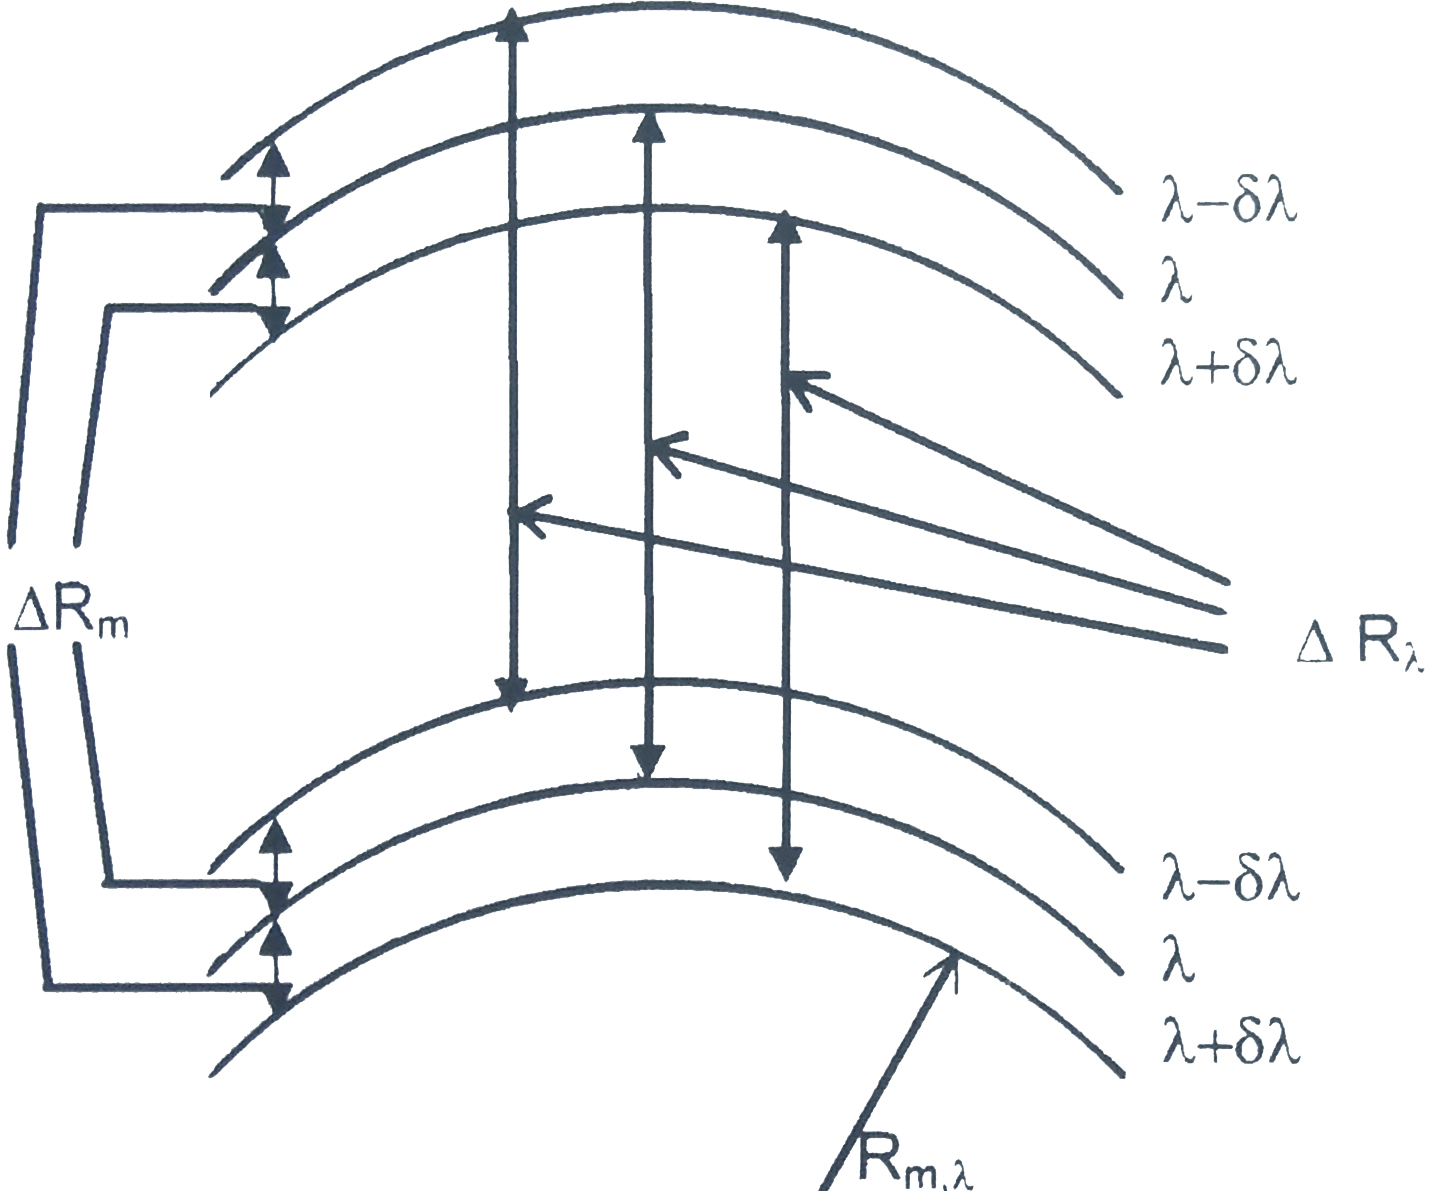
\includegraphics[width=0.7\linewidth]{fig/fig9.jpg}
	\caption{Вид двух соседних колец интерферометра Фари-Перо при расщеплении спектральной линии в магнитном поле. $\Delta R_m$ 
	- разность радиусов колец одного порядка интерференции, образованные излучением разных длин волн ($\lambda- \Delta \lambda, \lambda, \lambda+ \Delta \lambda$); $\Delta R_{\lambda}$- разность радиусов колец разных порядков интерференции, образованных излучением одной длины волны.}
	\label{fig:9}
\end{figure}

\begin{figure}[tb]
	\centering
	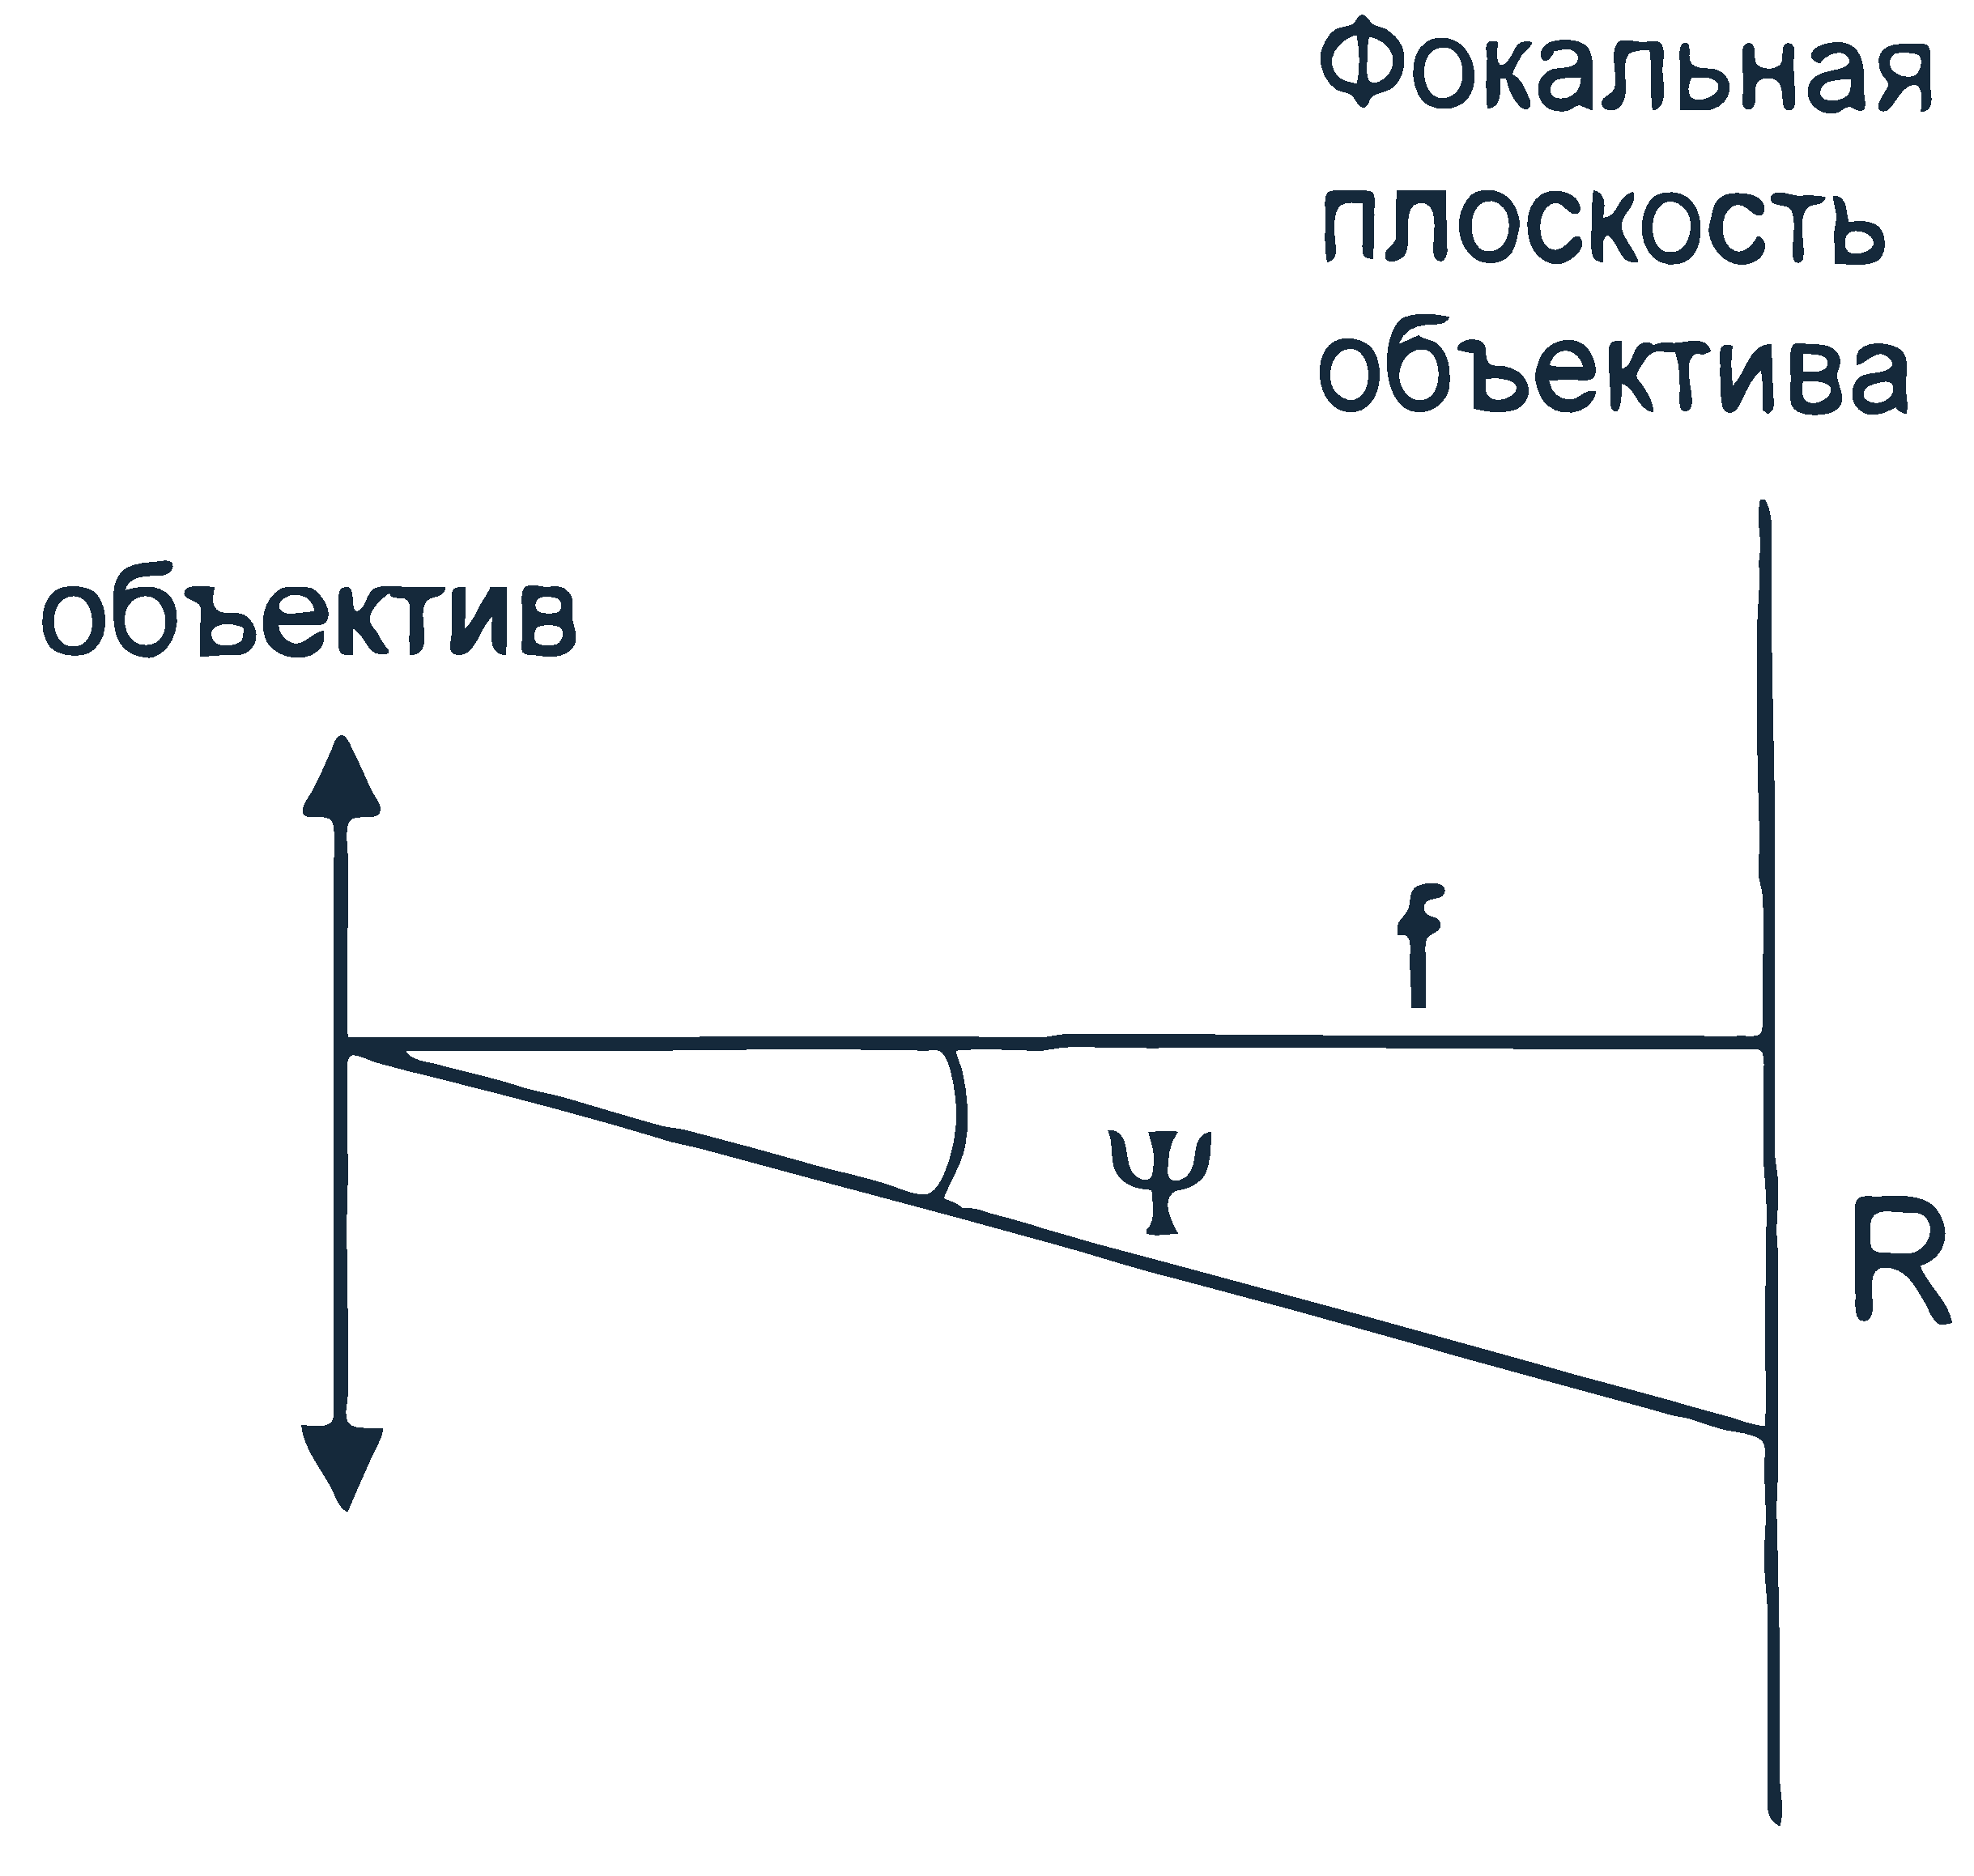
\includegraphics[width=0.5\linewidth]{fig/fig10}
	\caption{К расчету радиуса колец Фабри-Перо}
	\label{fig:10}
\end{figure}

% \begin{wrapfigure}{h}{0.4\textwidth}
% 	\centering
% 	\vspace{-50pt}
% 	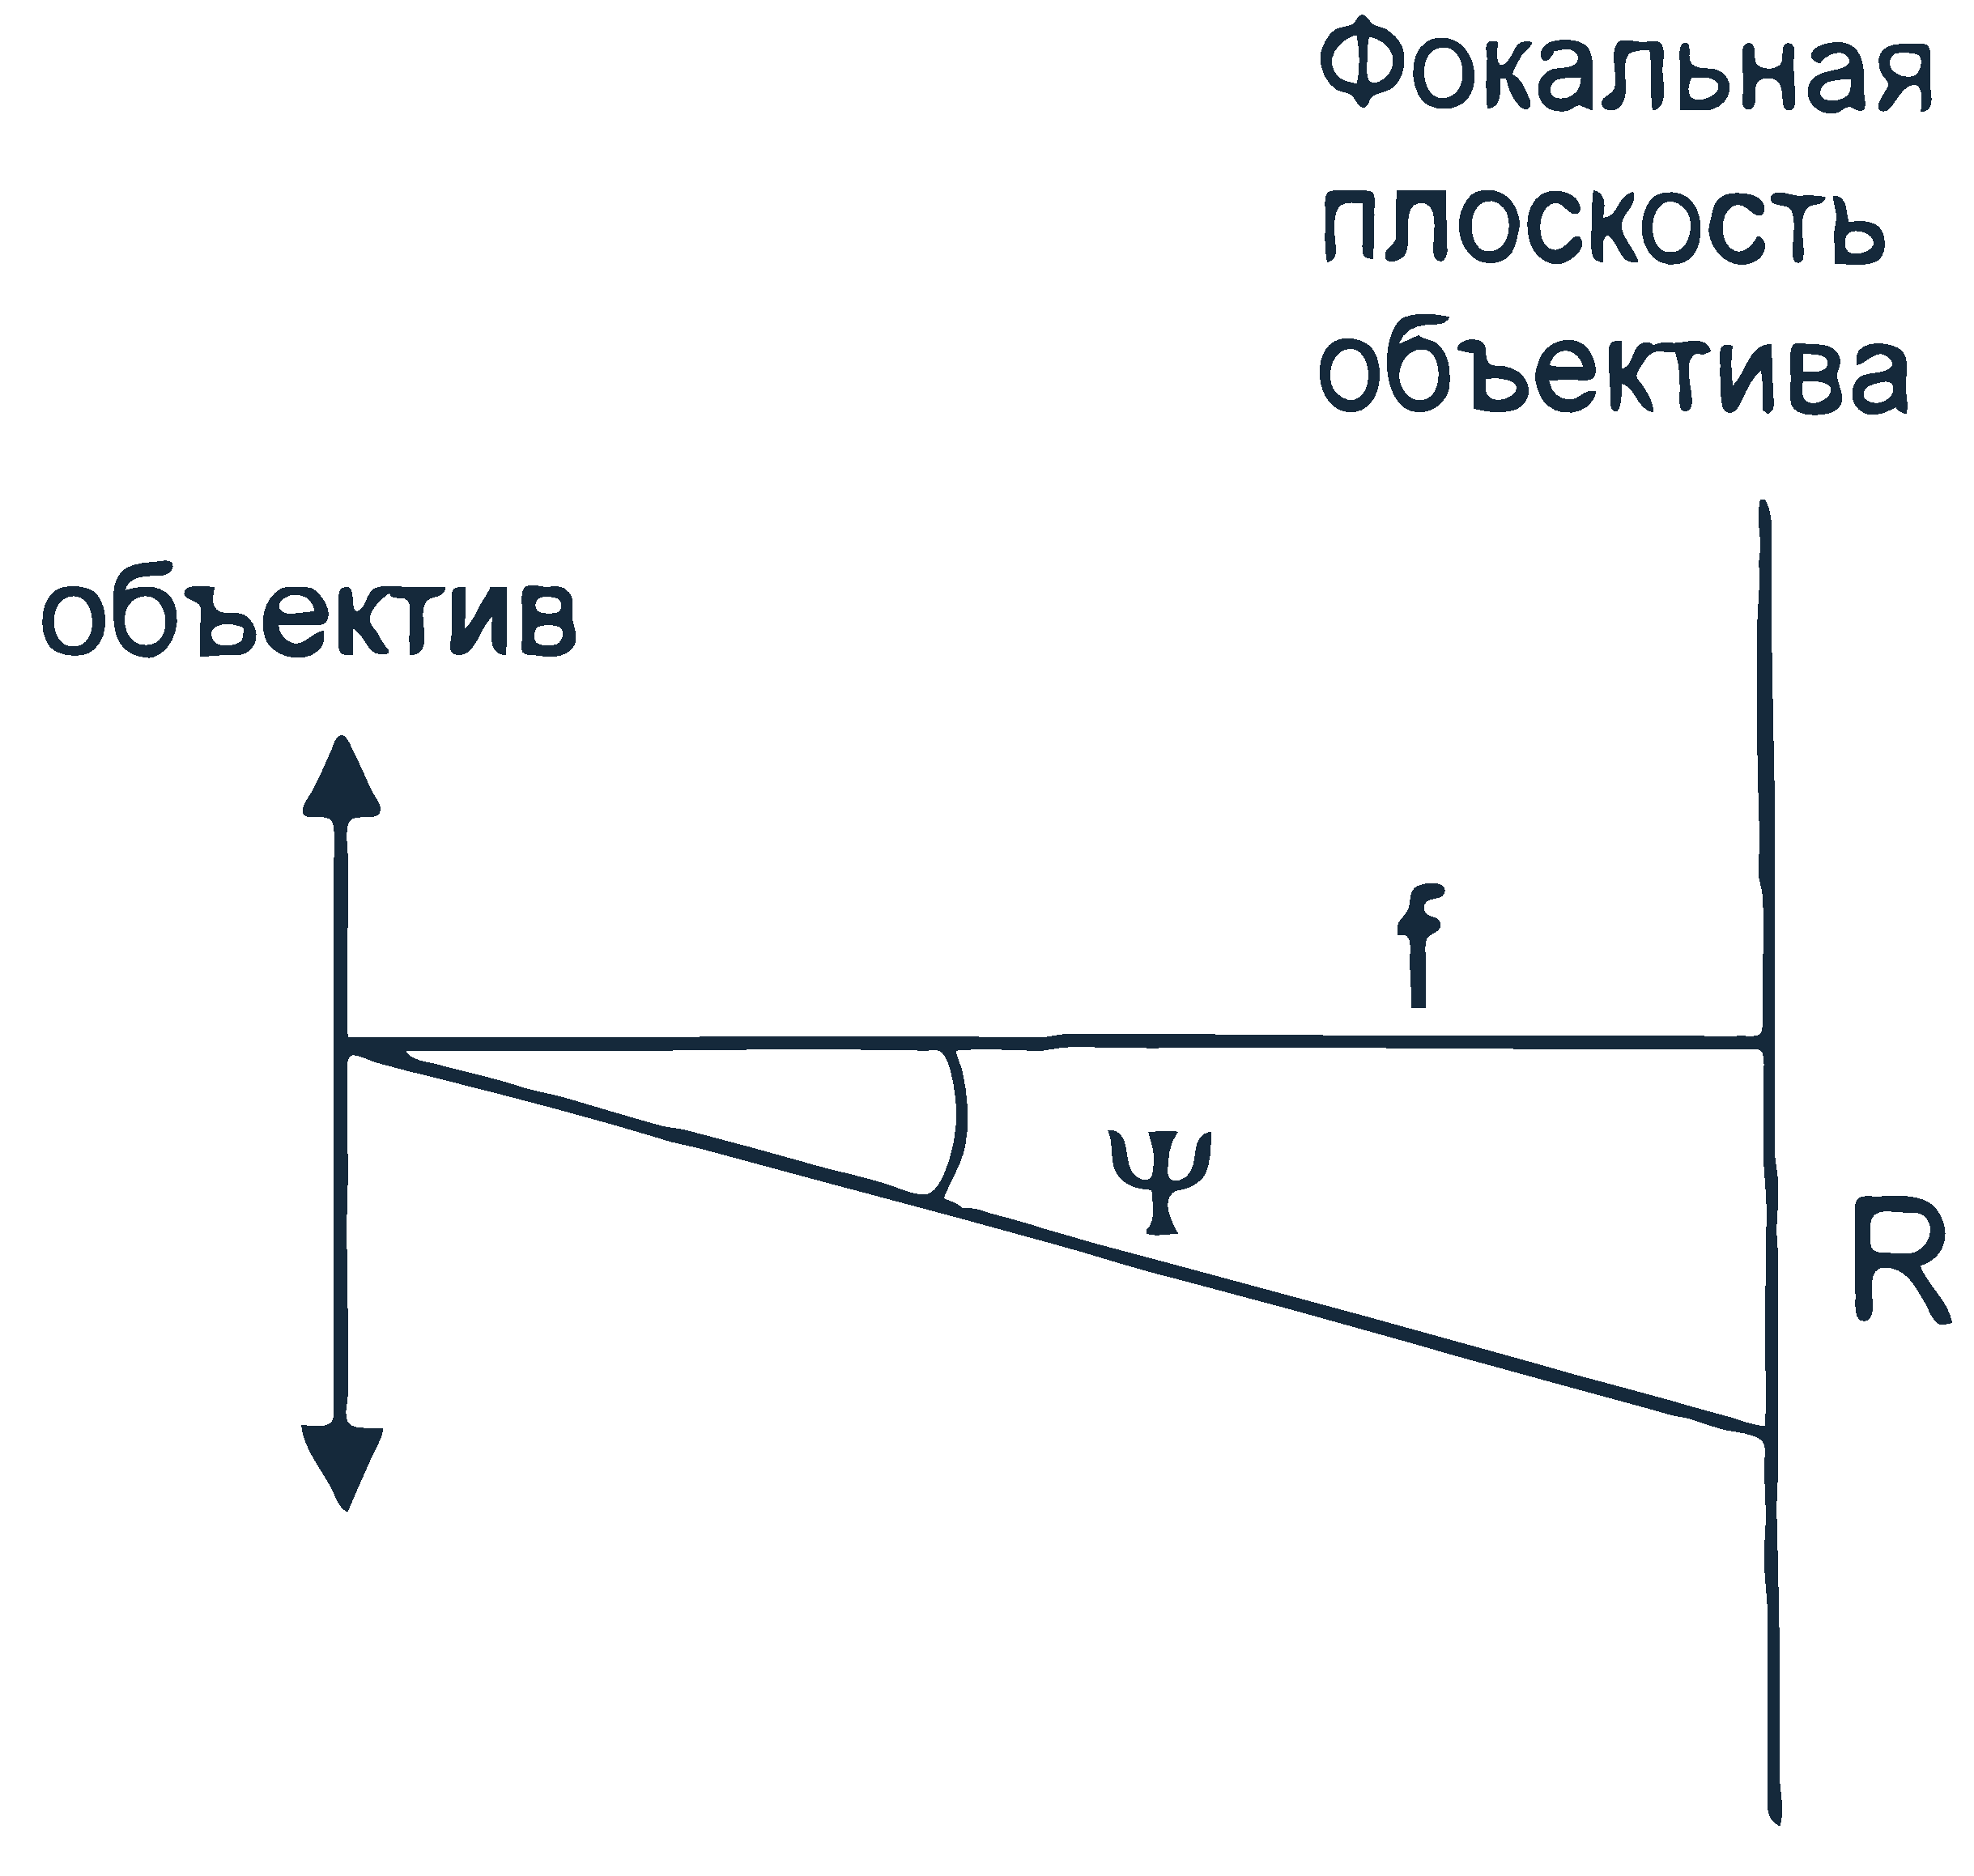
\includegraphics[width=\linewidth]{fig/fig10}
% 	\caption{К расчету радиуса колец Фабри-Перо}\vspace{-45pt}
% 	\label{fig:10}
% \end{wrapfigure}
%рис 10
Величину  разности углов $\delta \Psi_m$ и $\delta \Psi_{\lambda}$ найдем из \ref{eq:24}, которое с учетом малости $\Psi$ примет вид
\begin{gather}
	\label{eq:31}
	1-\frac{\Psi^m}{2}=\frac{m\lambda}{2h}
\end{gather}

Откуда получаем значения 
\begin{gather}
	\label{eq:32}
	\delta \Psi_m=\frac{m\delta \lambda}{2h\Psi_m} и \delta \Psi_{\lambda}=\frac{\lambda}{2h\Psi_{\lambda}}
\end{gather}

Усредняя результаты измерений,получим
\begin{gather}
	\label{eq:33}
 	\langle \Delta R_m \rangle  = f \langle\delta \Psi_m\rangle =f\frac{m\delta \lambda}{2h}  \langle\frac{1}{\Psi_m} \rangle
\end{gather}

Аналогично для
\begin{gather}
	\label{eq:34}
	\langle\Delta R_{\lambda}\rangle  = f \langle\delta \Psi_{\lambda}\rangle =f\frac{\lambda}{2h}  \frac{1}{\Psi_{\lambda}} 
\end{gather}

Из соотношений \ref{eq:33} и \ref{eq:34} с учетом равенства $ \langle\frac{1}{\Psi_m}\rangle = \langle\frac{1}{\Psi_{\lambda}} \rangle$, 
которое следует из того, что углы $\Psi_m$ и $\Psi_{\lambda}$ принимают один и тот же ряд значений, получим формулу для расчета $\delta \lambda$:


% \begin{equation}

% 	\langle \Delta R_{\lambda} \rangle=
% 	\frac{m \delta \lambda}{\lambda},
% \end{equation}

% полагая $m=\frac{2h}{\lambda}$, получим

\begin{equation}
	\label{eq:35}
	\delta \lambda = \frac{\lambda^2}{2h} \frac{\langle \Delta R_m \rangle}{\langle \Delta R_{\lambda}\rangle}
\end{equation}

% Регистрировать данные измерений и производить их обработку удобно, используя таблицу \ref{tab:3}, где $ \langle \Delta \rangle R_m  = \frac{1}{4} \sum^4_{i=1} \Delta R_mi$, $ \langle \Delta  R_{\lambda} \rangle = \frac{1}{3} \sum^3_{i=1} \Delta R_{\lambda i}$